\documentclass{report}

\usepackage{amsmath}
\usepackage{graphicx}
\usepackage{hyperref}
\usepackage{cleveref}

\graphicspath{ {./figures/} }

\begin{document}

\title{Scale- and Translation-Invariant Unsupervised Learning of Hidden Causes Using Spiking Neurons with Selective Visual Attention}
\author{Youssef Kashef\\
\\
\\
Submitted in Partial Fulfillment of the Requirements\\
for the Degree of Master-Diplom\\
in Neural Systems and Computation\\
at\\
ETH Z{\"u}rich\\
\\
}
\date{7. August 2013}

\maketitle
\tableofcontents

\begin{abstract}

Nessler et al. have demonstrated the ability of a spiking neuronal network governed by spike-timing-dependent-plasticity (STDP) and a stochastic winner-take-all (WTA) circuit to learn and predict causes from visual input. We aim to increase the computational power of the existing network through invariance to translation and scale. The visual system of the brain masters the recognition of objects wherever they appear in the visual scene, regardless of scale, orientation or even with partial occlusions. It achieves this through attention. Therefore, we turn to the pool of literature on modeling visual attention systems inspired from the brain. The architecture of the extended model is composed of the existing recognition module receiving bottom-up input from an attention module. Pre-attentive computations allow the attention module to alter the input window exposed for recognition. Attention is modeled as a network measuring for saliency in a scene by feature extraction with the use of hierarchies. The design and development of this extended model to achieve the required invariance by using processes that approximate their biological counterparts is presented. Emphasis is put on making these approximations through computationally economic implementations. Evaluation of the model is based on its performance and convergence in a set of experiments as well as its computational efficiency. Experiments are constructed to scrutinize the behavior of the model, its ability to converge onto a sight within a scene that enables recognition. Artificial as well as natural images are used to further reveal the capabilities and limitations of our approach. A top-down feedback signal of the recognition module that modulates attention is discussed.

\end{abstract}

\chapter*{Introduction}

\paragraph{}\textbf{Spike-based Expectation Maximization (SEM)} is a model of bayesian modules articulated by Nessler et. al of how the brain analyzes sensory stimuli. The model demostrates the learning of hidden causes in visual stimuli emerging through correlations in a stochasitc soft winner-take-all (WTA) network of spiking neurons. The spiking neurons are activated continuously in the presence of their preferred stimulus \cite{Nessler2010}. Spike-timing-dependent-plasticity (STDP) in WTA circuits defines the learning method for recognizing the hidden causes in the stimulus. The utilizaton of STDP acts as an approximation of traditional Expectation Maximization \cite{Nessler2013}. This model forms the basis of the presented work.

More emphasis will be put on how the WTA circuit in the SEM model is constructed and utilized. This WTA circuit constitutes our main building block. It comprises of a feed-forward single layer spiking neural network. The input layer is made out of spiking nodes whose firing activity is governed  by a poisson process. External variables undergo a population coding that determines the modality of this poisson process. In the example offered by Nessler et al, the external variables are intensity values, pixel values, form a static visual stimulus, an image. The population coding polarizes the pixel intensity values into binary On-Off states which directly determine the firing probability of the poisson process. A spiking neuron is assigned to encode each state of the population code generated for each pixel. In this case, two spiking nodes per pixel. An On-node and an Off-node. The firing rate of these neurons is proportional to the state of the node in the population code \cite{Nessler2010}.

\paragraph{}\textbf{Selective Attention} delivers a strategy to economize computational power and reduce its entropy. Its evolutionary motivation comes for the organism's need to detect prey rapidly. Itti et al. propose a framework for attention involving interactions between bootom-up cues that are stimulus driven and top-down cues that are task-dependent \cite{Itti2001}. The bottom-up cues are triggered by a mechanism for static feature detection and possibly also temporal event detection. Top-down attention may originate from predictive mechanisms that bias selectivity. Top-down cues may also arise from indepdendent motor control \cite{Olshausen1993}.

Extending the SEM model with feature-based modules and providing input that is previously filtered by an attention module we demonstrate a reduction in dimensionality, increase in computational efficiency and invariance to scale and translation.

\chapter{Methods}
\section{Object Recognition using Spike-based Expectation Maximization}

\subsection{Extending SEM by learning orientations}

The original SEM model is made out of an input layer receiving signals from external variables $x$. Population codes determine the state of a set of spiking neurons $y$ for each node $x$. The spiking pattern of each node $y$ follows a poisson process. Spikes generated from all $y$ neurons serve as input to a WTA circuit of $z$ neurons with weights \textbf{$w$} for each neuron. The $z$ neurons form the output layer. The use of notations $x$, and $z$ is to draw the connection to the Expectation Maximization algorithm that the model approximates. As it tries to maximize $E_p*[log \hspace{5 pt} p(y|\textbf{w})]$ with $q(z|y)=p(z|y,\textbf{w}^{old})$ in the E-Step, where $\textbf{w}^{old}$ is the weight vector for each of the $z$ neurons and replacing \textbf{$w$} with updated weights for the M-step \cite{Nessler2010, Nessler2013, Habenschuss2013}.
Applied to an example, $x$ variables are pixels from a static image of a handwritten digit. Two $y$ neurons fire antognistically, depending on the intensity level of their associated $X$ node (where $X\in x$). Nurons in the $z$ layer produce a firing pattern that is distinct for to the hidden cause. The handwritten digits can be categorized into distinct classes and we see that the SEM can produce a unique firing pattern for each class through unsupervised learning \cite{Nessler2010}. 

\paragraph{}We will keep the WTA circuit as our main building block. We will also preserve the hebbian learning rule to update the weights of $z$ neurons to use for the M-Step \cite{Nessler2010}. The population coding for polarizing intensity values to drive the poisson process will remain useful, but the population coding will also be the first entry point for the extension.

The current encoding of external variables accounts for the intensities of the spatial units, pixels, of the presented stimulus. The encoding of intensities is performed through a population coding by antognistic binary nodes per pixel that drive a poisson process \cite{Nessler2010}. Parallel to these intensity encoded nodes, we add a WTA circuit per pixel that determines the preferred orientation of this node relative to its spatial neighbors. This creates an orientation map of the presented stimulus. Whilst counter-intuitive with traditional learning models, SEM benefits from elaborating the dimensionality of WTA's feature space as this increases its resolution for detecting correlations between an output node $z$ and input nodes $y$ on a linear scale. Since SEM aims to reduce dimensionality, it is preferable to describe it as an elaboration of dimensionality. The added dimensions, or nodes, do not carry new information, but rather refine its representation. Recalling the use of using population coding to encode in atagonistic (On-node, Off-node) fashion, thus letting the WTA learn the likelihood of an input node firing and not firing explicitly, as shown by \ref{eqn_corr}.

\begin{equation}
	p(z=1|y) \propto y*p(y=1|z) + (1-y)*p(y=0|z)
	\label{eqn_corr}
\end{equation}

where
\begin{itemize}
  \item $z$ denotes an output node,
  \item $y$ denotes an input node
\end{itemize}

As we introduce the orientation map we add additional operands to \ref{eqn_corr} to account for the node's preferred orientation.

\begin{equation}
	\begin{split}
		p(z=1|y_I \cup y_O) \propto &y_I*p(y_I=1|z) + (1-y_I)*p(y_I=0|z) \\
			&+ y_o*p(y_O=O_p|z)+\sum_{i\neq o_i} (1-y_O)p(y_O=o_i|z)\\
	\end{split}
	\label{eqn_corr2}
\end{equation}

where
\begin{itemize}
  \item $y_I$ denotes an input intensity node,
  \item $y_O$ denotes an orientation input node,
  \item $O$ denotes the set of orientations available. Orientations can be defined discretly and arbitrarily (e.g. 30, 60,...180 degrees) or they can be learned \cite{Nessler2010},
  \item $O_p$ denotes the preferred orientation
\end{itemize}

We redesign the network with a cascade of hierarchical WTA circuits. The input layer is a matrix of WTA circuits per pixel. Each input WTA circuit decides on the preferred orientation and intensity of its input. We will experiment with configuring the input WTA circuit to only relay intensity, or only orientation as depicted in \cref{fig:network_learn_orientations}, or both information.

\begin{figure}[ht]
\centering
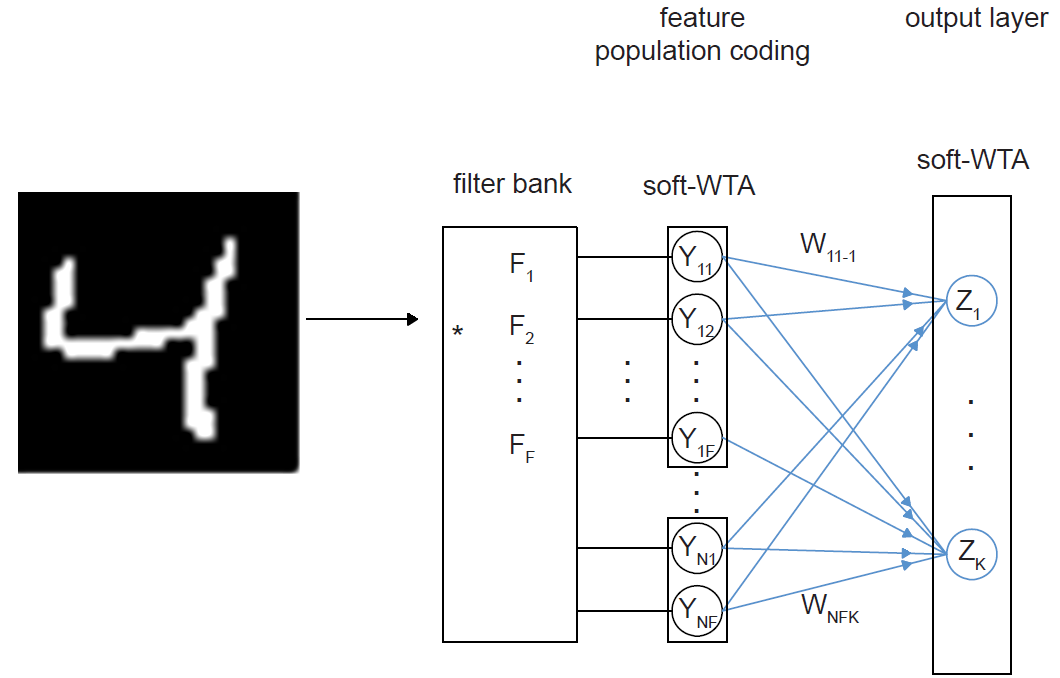
\includegraphics[width=0.8\textwidth]{network_learn_orientations}
\caption{SEM extended with a filter bank and an orientation discriminating WTA circuit for learning an orientation map of a visual stimulus. \label{fig:network_learn_orientations}}
\end{figure}

\begin{figure}[ht]
\centering
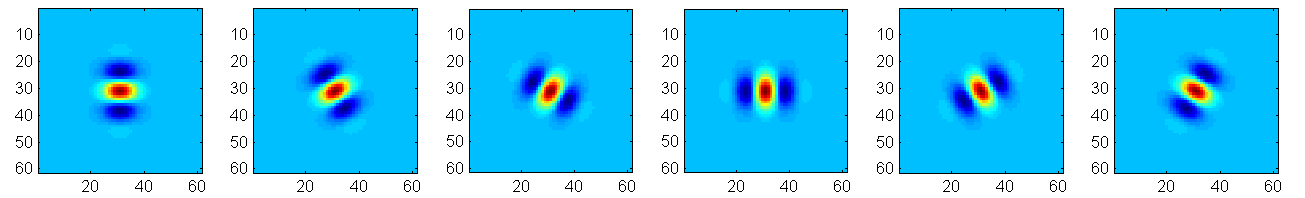
\includegraphics[width=0.8\textwidth]{filters_real}
\caption{Example of Gabor filters (real part). Defined at orientations [0, 150] degrees with increments of 30 degrees. \label{fig:filters_real}}
\end{figure}

The WTA circuits responsible to determine the preferred orientation of all input nodes are activated by convoling the stimulus with a bank of two-dimensional Gabor filters. The filters are defined with different scales and angular orientations from a predefined discrete set. \Cref{fig:filters_real} provides an illustrative example of such Gabor filters. By comparing the magnitude of responses between the filters at each pixel we can decide on the pixel's preferred orientation. Talking about the preferred orientation of a single pixel does not actually carry much meaning. The transfomations do yield responses for each pixel but they only become informative in relation to the responses of its neighbors. Examples of filter responses to a binary image stimulus are shown in \cref{fig:response4}

\begin{figure}[ht]
\centering
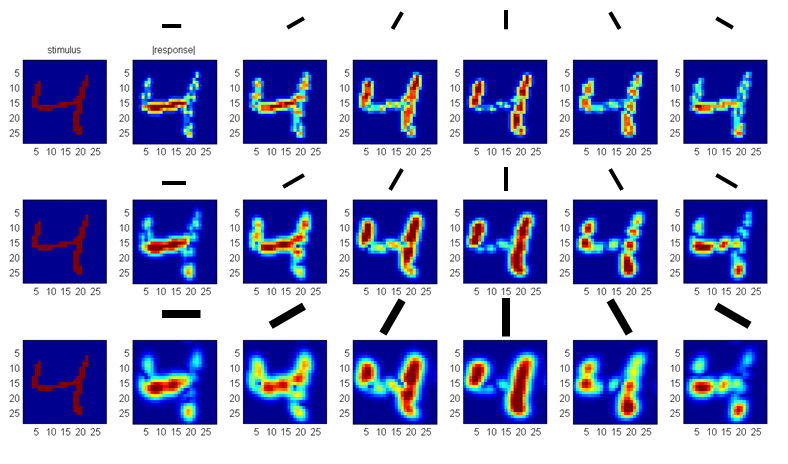
\includegraphics[width=0.8\textwidth]{response4}
\caption{Example of filter response magnitudes when convoling a binary image with Gabor filters defined at different scales and orientations.
\label{fig:response4}}
\end{figure}

Parameterized Gabor functions are an adequate approximation of simple cells in the primary visual cortex \cite{Serre2004}. Daugman demonstrates the construction of a neural network to achieve this transformation \cite{Daugman1988}. However, this work adopts the traditional systems' approach for defining and applying the filters.

\subsection{Extending SEM by learning hidden features}

We have seen the computational power of the SEM model as an unsupervised method for identifying hidden causes. So far the hidden causes have been used synonymously with predefined classes (e.g. numerical digits from the MNIST database \cite{LeCun1998}). We extend the SEM model in a way that breaks this assumption. We insert an additional layer, a WTA circuit, responsible for learning hidden causes that depict abstract features of the object we attempt to detect and recognize. This feature layer will contribute to the bottom-up learning as we expose it to the low-level input and and have it drive the WTA circuit already encountered in the original SEM architecture. With this additional feature-WTA circuit introduced, we no longer require presentation of the entire stimulus but will restrict stimulus presentation to subregions within the space of a stimulus. These subregions may represent salient regions within a stimulus. The definition and method of selecting these subregions will be discussed in more detail as we discusss the object detection module.

\section{Towards Object detection using visual attention}

\subsection{Achieving invariance}

\paragraph{}Itti et. al anchor their bottom-up computational model of attention as a saliency search within a visual scene. They demonstrate how attention is achieved in an image based environment. The image is evaluated for conspicuities in features such as illumination, color, texture or other. The feature extraction is pre-attentive. A spatial map of each feature at different spatial scales is unified into a single conspicuity map for this feature. The conspicutiy maps are combined linearly into a saliency map of the image. The saliency map represents a reconsiliation of the pre-attentive features as the magnitudies need to be normalized before we can can combine them. The saliency map seeds the search to locate visual objects in a scene. The objects can later be processed for recognition with less computational overheads \cite{Itti2000, Itti2001}.

The above saliency mechansim defines the distribution from which we sample windows of attention. The windows of attention are forwarded to the recognition module as a continuous feed of input. Itti et al. emphasize that their model does not cover any top-down attention components, yet they address the importance of preventing the 'focus of attention from immediately returning to the previously-attended location' \cite{Itti2000}. This is expected to happen in a purely bottom-up method as the saliency value remains constant. Therefore, we need to bias the model to attend to the second-most-likely salient location. Since we are using windows of attention as input to a recognition system, inhibition of return (IOR) enables such input to be more diverse. The proposed mechanism for IOR, adopted fro Itti et al is the convolution of the saliency map with a Off-centre-On-urround kernel that inhibits the centre located on top of the previous window of attention and enhances the saliency of its surroundings. Itti et al. point out that the effect of IOR should remain transient and need only be maintained temporarily \cite{Itti2000}.

\paragraph{}Olshausen et al.'s earlier attempt to formalize a framework for attention includes the concept of bottom-up flow of information before attempting recognition but also mention the presence of a top-down mechansim intercepting the signal. This mechanism arises from "control-neurons" that dynamically modulate synapses, or weights, for routing a selected spatial window from lower levels in the visual system to higher ones \cref{Olshausen1993}. They describe how scale-invariance is achieved through magnification of the window of attention to fit a "canonical reference window". This concept is computationally equivalent to resizing an image via interpolation leading to a blurred appearance of the attended window inside the reference frame. Their control units come into play as they can shift the window of attention up or down scale levels or translate within a single plane, scale. This conscious control represents behavioral control of attention that can arise from motor control. This motor control can be voluntary or not, however the authors are more focused on the case of involuntary control. To demonstrate the employment of the same control neurons as part of a closed-loop autonomous system, Olshousen et al. describe a strategy that governs these control units.
This strategy is made out of:
\begin{itemize}
  \item Low-pass filter the visual scene into blobs.
  \item Point the reference window to the location of the blob, adapting to its topography (i.e. size and location).
  \item Pass original input represented by the blob to the recognition module.
  \item Assess match of the presented object with previously learned objects. Take action according to recognition results (e.g. learn as a new object, discard it, perform a task, etc.) \cite{Olshausen1993}
\end{itemize}
The authors provide an elaborate derivation and description of this model. We see them taking the initial steps of what we learn from Itti's salient-based model in addition to the notion of turning the open-loop system into a closed-loop one through the feedback signal of modulatory control neurons whose activiy is a relay of the response of a recognition module. However we encounter some gaps in how some of the intermediate steps of modulation are defined, as these may depend on application or the recognition module itself, how it operates, how it responds. 

\paragraph{}A computational model of top-down attention is proposed by Baluch et al. The top-down model is described as a mechanism that influences the stimulus drive generated from the familiar bottom-up mechanism. The influences come in the form of feature bias, spatial bias, context or a task being carried out. These same influences can generate an attention field independent of the stimulus drive. The attention field and modulated stimulus drive are multiplied and normalized to yield a response to apply detection on. An analogous top-down attention model is presented that involves a learned approach. A learner is presented with bottom-up derived features to predict top-down saliency. Top-down saliency is multipled by bottom-saiency to form a unified priority map over the visual space \cite{Baluch2011}. This model provides a concise interaction of bottom-up and top-down mechanisms, thus bridging bridging Itti et al's with Olshausen et al's frameworks.

\paragraph{}The SEM model requires some extensions to achieve scale- and translation invariance. Scale invariance can be achieved through the use of intermediate layers that learn features of visual objects that are more abstract than pixel intensity values. We can predefine these features in the form of orientation maps. It is also possible to let the SEM model learn abstract features driven by the stimuli. The features can be pre-extracted using decimated versions of the orginal visual stimulus, thus reusing existing neurons in the network as if they were with enlarged receptive fields. We expect that these abstract features can pick up simple shapes such as oriented bars as well as more complex shapes. The network wiring will emerge from the features extracted by the data and the interactions within the stochastic processes within the SEM. The model will become invariant to XY-plane translations through the use of selective visual attenion. Bottom-up saliency-based attention is employed following the model proposed by Itti, Koch and Niebur \cite{Itti2000}. The introduction of a top-down component can be made by using the spikes of the output layer as a feed-back signal to modulates attention.

\subsection{Feature-population coding}

Towards invariance to translation we employ Itti et al.'s bottom-up saliency-based attention mechanism. It serves the purpose of locating regions within a visual scene to present to the network. Population coding will be used for encoding an analog and/or binary state of a neuron, $y$ neurons, into spike trains. The state of these neurons will be derived from pixel intensity values, binary, and analog filter responses when convolving salient regions with filters from a predefined filter bank. Population coding derived from filter responses will be referred to as feature population coding. The original simple population coding and feature population coding generate input to the new network iluustrted in \cref{fig:fig_network}.

We refer to the original population coding as 'simple' because it operates directly on the bi-state external variable and only generates spikes that elaborate on these two states. The feature popluation coding investigates the use of a soft-WTA circuit to determine the state of the spiking neuron in a population \ref{fig:network_learn_orientations}. The population represents a set of feature states and the soft-WTA circuit determines the dominant state(s). In this case the population represents the response of a node after convolving the stimulus with a bank of Gabor filters. The WTA circuit draws the preferred orientation from the stochastic process whose distribution is defined by the analog response to each filter. The use of winner-take-all circuits correlates with the HMAX framework \cite{Serre2004, Riesenhuber1999}. Employment of the soft-max operator allows for a representation of intermedia features (i.e. an angular orientation that lies between two states in the predefined set). It also provides good mitigation against local maxima during the learning process.

\begin{figure}[ht]
\centering
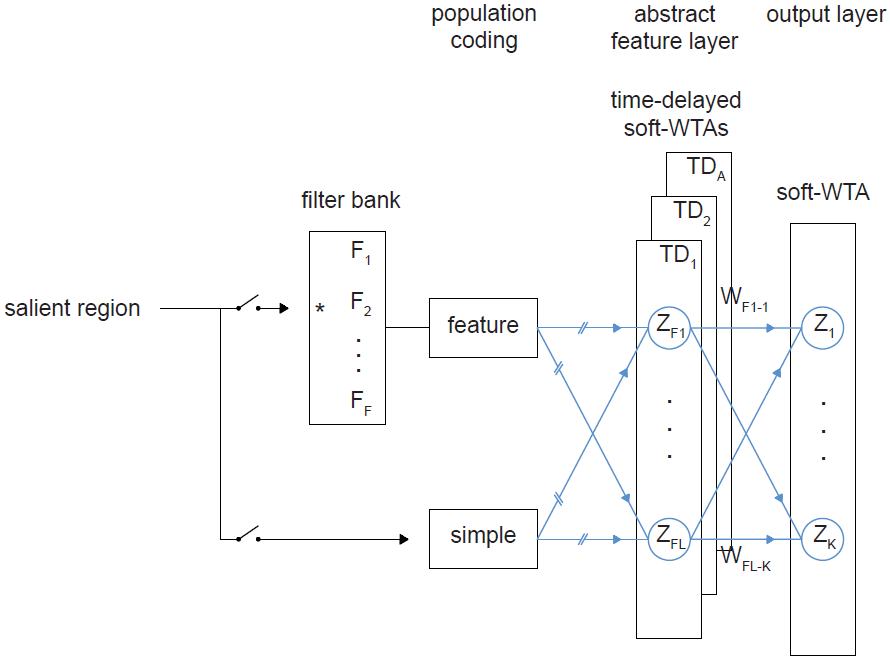
\includegraphics[width=0.8\textwidth]{network}
\caption{The network with which SEM is extended. The network is composed of multiple layers, namely a layer of spiking $y$ neurons that are stimulated by intensities and filter responses of the presented salient image region, a layer of $z$ neurons inside a WTA circuit that learn the patterns presented to them which will be referred to as the $f$ layer, or $f$ neurons, and finally the WTA circuit of $z$ neurons that learn the spiking pattern of the $f$ layer in a familiar and equivalent WTA fashion.
\label{fig:fig_network}}
\end{figure}

The bottom-up attention mechansim employed is a varied implementation of Itti et al.'s model. Their model defines a salient-based mechanism to evaluate a visual scene on location worth attending to.
The commonalities between this intepretation and the original model are:
\begin{itemize}
  \item the use feature maps based on intensity and orientation,
  \item detecting conspicutity from center-surround differences,
  \item normalizing feature conspicuity maps to combine them into a single saliency map.
\end{itemize}
As for differences, unlike the original model, this intepretation:
\begin{itemize}
  \item use feature population coding, Gabor filter transformations with soft-WTA circuits, instead of linear filters,
  \item omits color feautres, focusing only on binary image stimuli,
\end{itemize}

\subsection{Learning abstract features}

The attention mechanism provides a continuous feed of subregions in the original stimulus space that may contain patterns worth learning for recognizing objects. This can happen whether the attention mechanism is a purely stimulus-driven or modulated by top-down cues. We are willing to restrict the input space used for training and testing the recognition system to patterns that qualify as salient. The SEM model treats such salient windows as its external variables $x$. Population coding, simple and feature-population coding, produces spike trains that represent the intensities in the pixels and their the orientation map of such a window. A layer of $z_F$ neurons interact within a soft-WTA circuit. These $z_F$ neurons employ the same learning rule. Their WTA-circuit is essentially the building block brought over from the original SEM model. This layer is described as the abstract feature layer, or F-layer, as it learns to disriminate the abstract features provided by the salient window input. The spikes emerging from the F-layer activate the $z$ neurons in the output layer. The output layer remains responsible for learning the hidden causes. Except that it now disriminates such causes in the distribution of abstract feautres, of far more reduced dimnensionality.

\begin{figure}[ht]
\centering
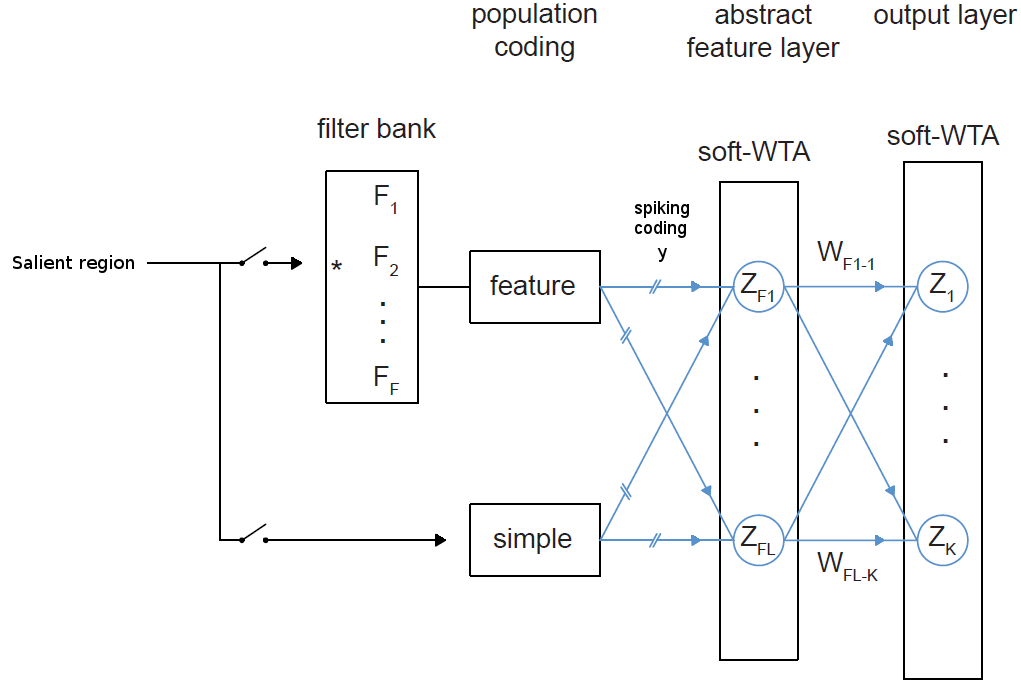
\includegraphics[width=0.8\textwidth]{architecture_recognition}
\caption{The architecture of the recognitiion module of the extended SEM model. The input is restricted to salient regions provided by the detection module via selective attention. The windows of attention is passed on to population coding, wheter simple bi-state coding of pixel intensity values or convlution with Gabor filters and WTA-circuit that discriminates the preferred orientation of the external variables. We will determine if the use of both population coding schemes are necessary or if only one is sufficient. Spikes generated from the population coding activate a soft-WTA circuit in the abstract feature layer, the F-layer. F-layer neurons learn patterns present in the window of attention. The neurons in the output layer learn hidden causes represented by the spiking distribution of the F-layer. 
\label{fig:architecture_recognition}}
\end{figure}

\Cref{fig:network} illustrates the wiring of a spiking neural network responsible for recognizing hidden causes in visual objects. The causes are represented by spiking patterns of the output-layer neurons that discriminate the spiking pattern of preceeding neurons in an intermediate layer. Neurons of the intermediate layer responds to the presence of abstract features present in a series of windows of attention. With the presentation of stimulus a detection module employing selective visual attention generates this series of windows of attention which are encoded into spike trains through population coding. Population coding may be 'simple', based on pixel intensity values, more complex by evaluating the response of the sub image to filters, or both.\\
Here it becomes necessary to point out a predicament. Attention windows arrive at the recognition module serially. This does not cause any problems for the $z_F$ as the scope of their operation is within a single window of attention. However, in the case $z$ neurons in the output layer need a larger scope as their response needs to be associated with the original stimulus. A sophisticated solution to this problem is likely in the use of a memory modulem or state machine that preserves the state of the output layer for different windows of attention belonging to the same stimulus. Markov chains present a possible approach for maintaining temporal states. This may be achieved through the use of self-excitatory synapses for neurons in the output layer. As intriguing as this approach is, we opt for a system's approach to the problem through the use of TODO   
Time-delay components are needed to reconcile attention windows arriving at the recognition module serially while it is desired to present the F-layer,  For associating the response of $z$ neurons to stimulus we employ a time-delay component in the network. The time-delay component is represented by 

\begin{figure}[ht]
\centering
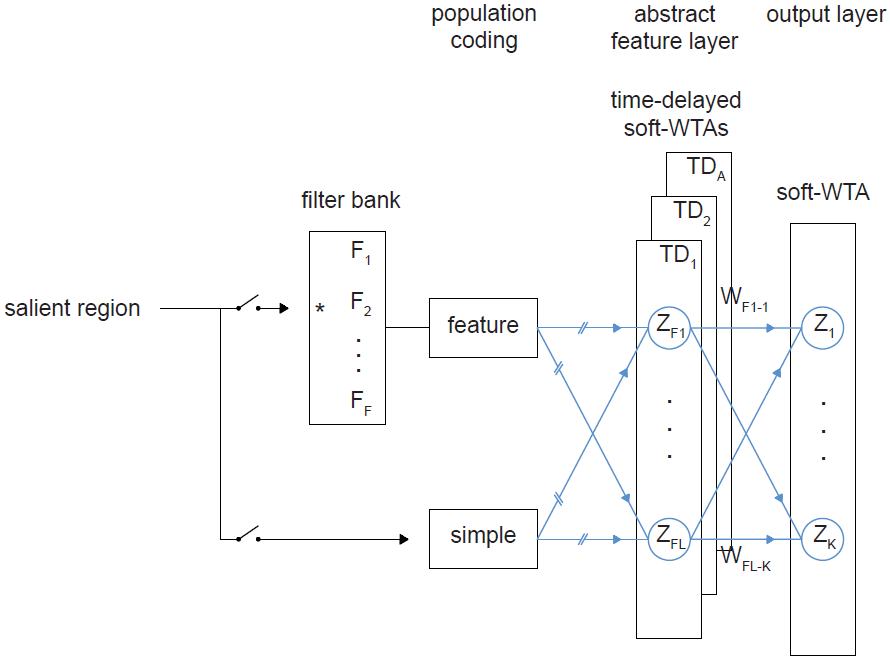
\includegraphics[width=0.8\textwidth]{network}
\caption{The network of the recognition module extending the SEM model. Input is provided by the attention mechanism in the form of windows of attention. Population coding encodes analog intensity or filter response values into spike trains which activate a soft-WTA circuit. Spikes generated from the $z_F$ neurons of the soft-WTA circuit in the abstract feature layer excite $z$ neurons in the output layer. $z$ neurons in the abstract feature layer are responsible for learning and predicting the abstract pattern in the window of attention. $z$ neurons in the output layer are responsible for learning spiking patterns of the preceeding layer associated with hidden causes in the orignal stimulus.
\label{fig:network}}
\end{figure}

\chapter{Results}

\section{Exploiting inherit noise of a stochastic process}

The first extension to the SEM network was to enrich the representation of the external variables $x$. Instead or in a addition to bi-state pixel values we convolve the image input with a set of Gabor filters. A WTA-circuit is appplied to the response of each pixel to the Gabor filters to determine its preferred orientation through a stochasitc process. The use of the stochastic process is not as noise-free as applying $argmax(y_i)$, where $y_i$ denotes the magnitude responses of pixel $i$. The $argmax$ operator would even align well with the HMAX paradigm presented in the works of Riesenhuber, Poggio and Serre\cref{Riesenhuber1999, Riesenhuber2000, Serre2004, Serre}. However we have found that the noise inherit in the stochastic process mitigates the computational pitfall of low magnitdue response vectors very well. To elaborate, parts of the stimulus with very low intensity values, will results in low magnitude response values for all filters in the filter bank. However the insignificant response vector for a pixel still yields a result from the $argmax$ operator. It will actually yield a near constant result. To avoid learners from learning this constant pattern that does not carry any true information, we need a mechanism to handle such low response values. The problem is not really in the response vector of all-low magnitudes. We can generalize the problem to pixel response vectors with high uniformity. We can still align this model with the HMAX model if we resort a stochastic process. The stochastic process is able to resolve high-uniformity, high entropy, distribution of pixel response vectors through its inherit noise. If a learner relies on such response vectors as weights, the spike trains coding the response vector will reflect the uniformity and the learning rule will yield accordingly uniform weight distributions for the corresponding pixel, leaving such weights computationally useless. We find that the weight vector associated with this pixel is as uniform as the response, thus with the use of a soft-WTA the contribution of this vector of weights for this pixel relative to the global weight vector of the learner is merely constant. Thus the membrane potential of this neuron will not experience fluctuations due to these weights but rather weights whose local vectors have low entropy. \Cref{fig:weightsPerOrientation} depicts the distribution of weights associated with different orientations after a learning process involving handwritten digits as stimuli. We find that outer areas with generally low intensity activity are high regardless of orientation.

\begin{figure}[ht]
\centering
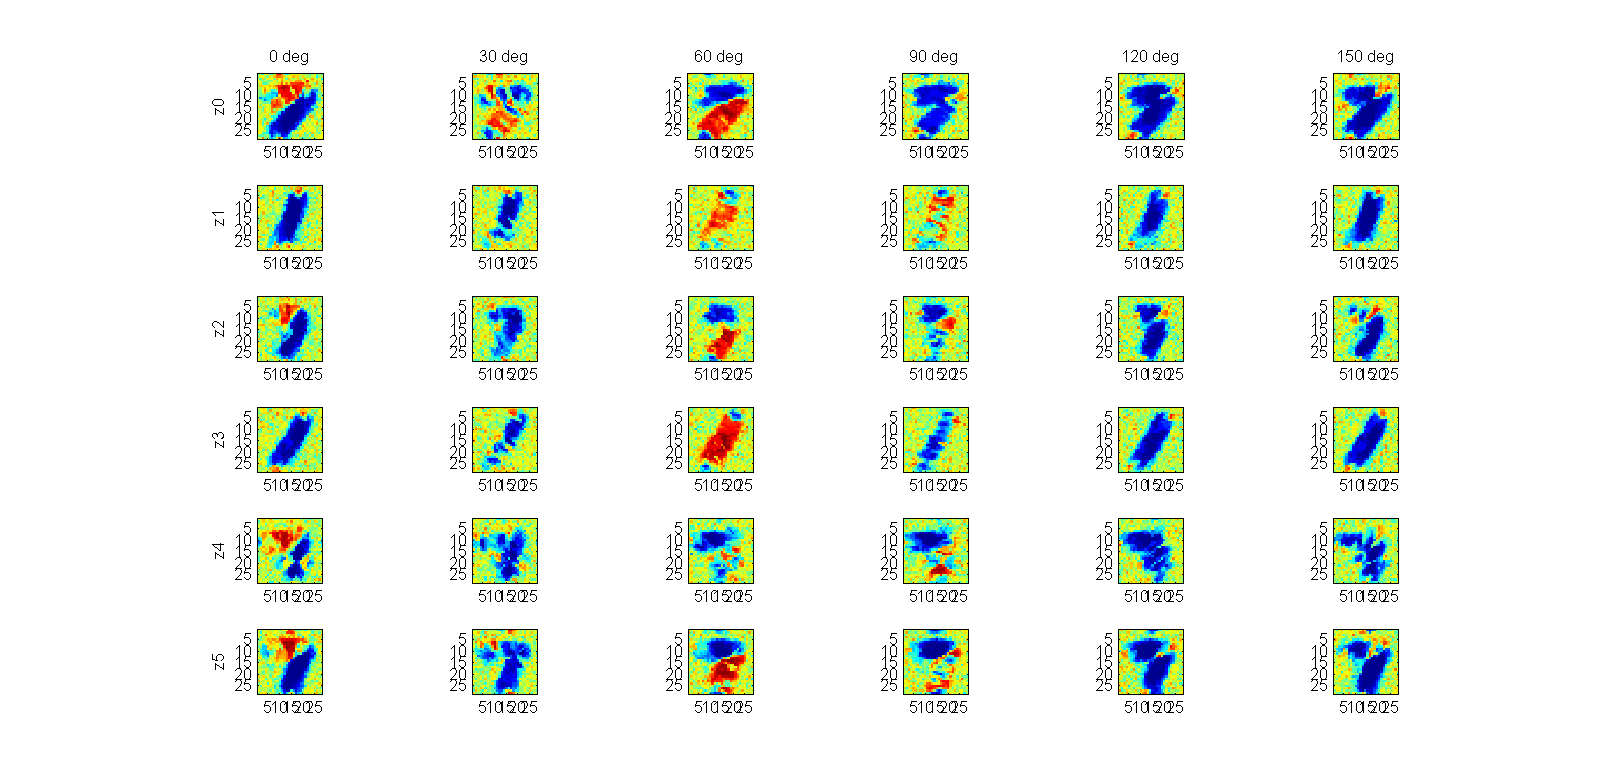
\includegraphics[width=0.8\textwidth]{weightsPerOrientation}
\caption{Example of $z$ neuron weight distributions for different orientations when using a hard max operator such as $argmax$ without accoutning for the uniformity of a pixel's response. Each row of subplots is reserved for a learner $Zi$, while each column is associated for an orientation. This is from an experiment involving handwritten variants of the digits 1 and 7 \cref{LeCun1998}. Blue colored regions have low weight values that yellow, orange and red, represent strong weights.
\label{fig:weightsPerOrientation}}
\end{figure}

If we picked the same weight from each orientation for the same learner, we'll find the distribution of this local weight vector to be fairly uniform. A local weight vector belonging to a pixel in an active region, will have some very low weight values for most orientations, and very high wiehgt values for fewer. \Cref{fig:weightCondEntropy} accomplishes this. It generates a local weight vector for each pixel, calculates its entropy to visualize the non-uniformity of the weights associated with each pixel in the XY-plane. Stimuli that activate weights belonging to a local weight vector with high netropy are a mere DC component in the resulting membrane potential of a neuron. While changing the input that invokes activity in weights belonging to low-entropy local distribution, will yield significant changes in that same neuron's membrane potential. \Cref{weightMaps47_masked} provides a more compact visualizations of the weight distribution by indicating the dominant weight, or preferred orientation associated with each external variable $x$ for different neurons $z$.

\begin{figure}[ht]
\centering
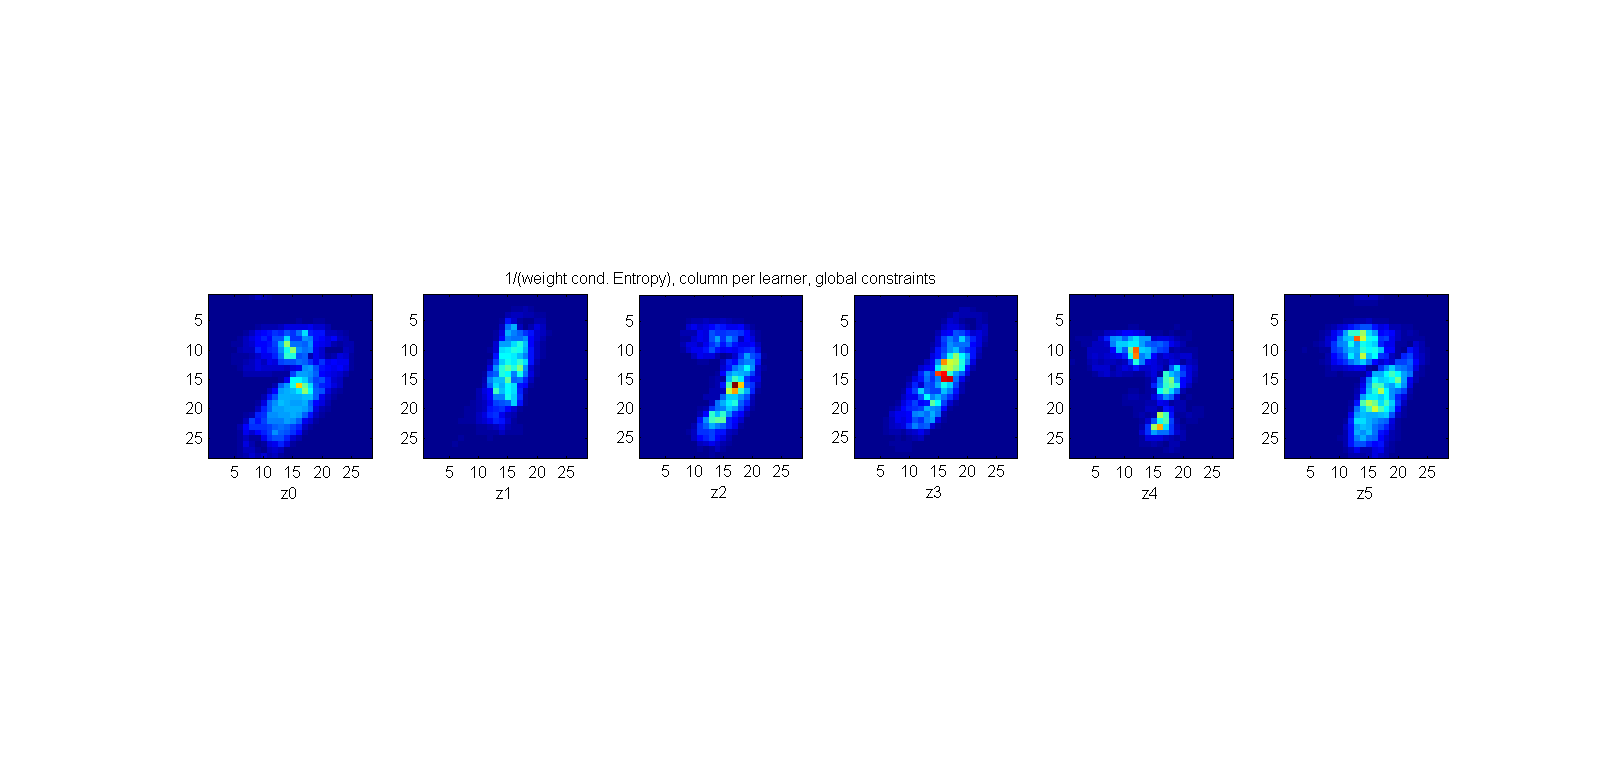
\includegraphics[width=0.8\textwidth]{weightCondEntropy}
\caption{Entropy of local weight vectors representing orientations associated with the same pixel. The intensity values in the image are anti-proportional to the entropy of the pixel's weight vector. This is from an experiment involving handwritten variants of the digits 1 and 7 \cref{LeCun1998}. Bright intensities are associated with low-entropy, strongly disriminating weight vectors, while low intensities are assoicated with uniform weight vectors whose contributions are merely DC components to the neuron's membrane potential. Each image represents this non-uniformtiy distribution of different learners.
\label{fig:weightCondEntropy}}
\end{figure}

\begin{figure}[ht]
\centering
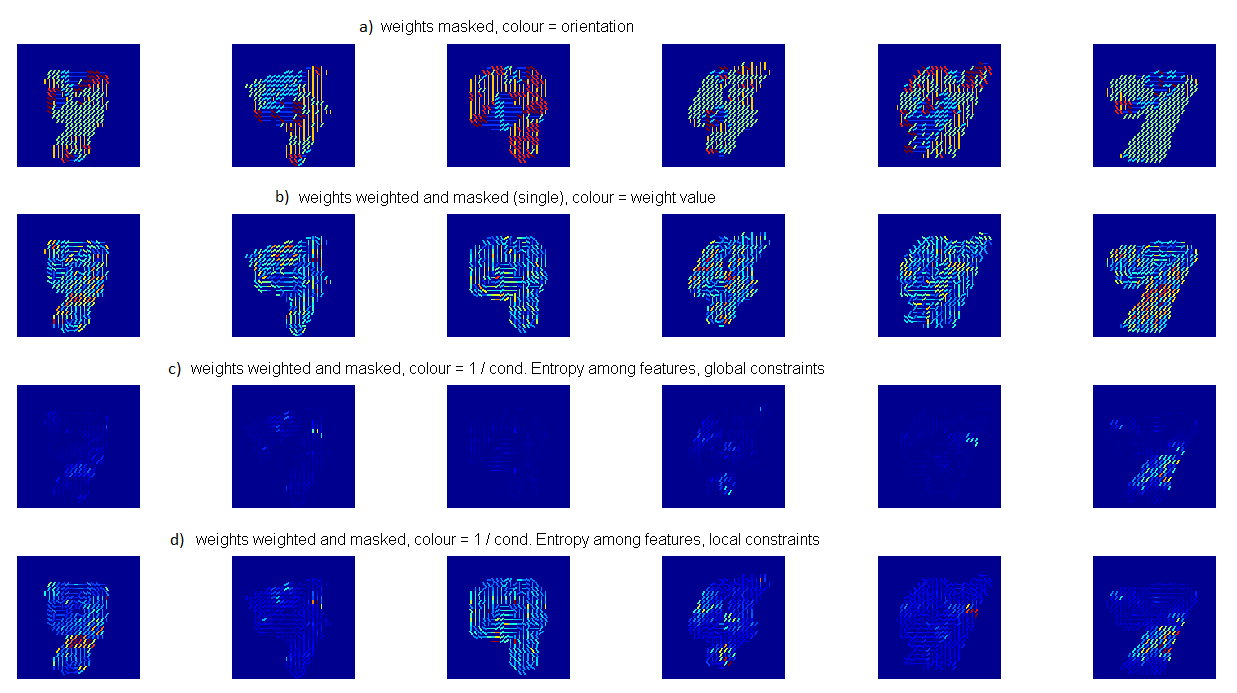
\includegraphics[width=0.8\textwidth]{weightMaps47_masked}
\caption{Visualizing weights of $z$ neurons after learning orientation maps of handwritten digits. Data used: a subset of handwritten digits from the MNIST database (classes 7 and 4) \cref{LeCun1998}, no overlap between training and test sets. Each column of images belongs to a $z$ neuron. The weight weight vectors have been reduced to two dimensional matricies by finding the dominant weight for each pixel. The preferred orientation of each pixel is determined via $argmax(\textbf{w}_x)$ where $X$ refers to the pixel and $w$ is the weight vector associated with this pixel. The length of \textbf{$w$} is proportional to the number of possible orientations defined. Regions of the image with very low intensity activity have been masked and appear plain while color represents  \textbf{a)} the preferred angular orientation of a pixel, \textbf{b)} the magnitude of the weight of the preferred orientation, \textbf{c)} the non-uniformity of a weight vector \textbf{$w_x$} normalized across all learners and \textbf{d)} the non-uniformity of a weight vector \textbf{$w_x$} normalized across the image. 
\label{fig:weightMaps47_masked}}
\end{figure}

\subsection{Measuring Saliency using feature-population coding}

Saliency is measured with the use of feature maps, one for intensity features and a second for orientation features. The intesnity feature map is generated by convolving the stimulus with a Difference of Gaussians for achieving centre-surround operations. Normal localization is applied on the filter response to empahsize conspicuities and a global normalization is applied on the entire feature map for later reconciling this itenstiy contrast map with other feature maps.  
The same stimulus is convolved with bank of Gabor filters. For each pixel the filter responses for that pixel are taken as input to a soft-WTA circuit. The soft-WTA circuit determines the preferred orientation of the pixel. Performing this for all pixels we generate an a map of the preferred orientation for each pixel, an orientation map. In order to detect conspicuities in these orientations we measure the distance of a pixel's preferred orientation relative to its neighbors and use the local variance of these diatance measures as a measure of concpicuity in orientation. The feauture map is then normalized globally and then masked for nodes with low magnitude responses to all filters before its use alongside the intensity contrast map.
The intensity contrast and orientation conspicuity maps are combined linearly into a single saliency map. Nodes in the saliency map with high response-magnitude indicate either high contrast, orientation conspicuity or both. The saliency map serves as a two-dimensional distribution from which we draw coordinates of locations worth attending to. \Cref{fig:saliency_examples} depicts examples of saliency maps evaluated for static images.

\begin{figure}[ht]
\centering
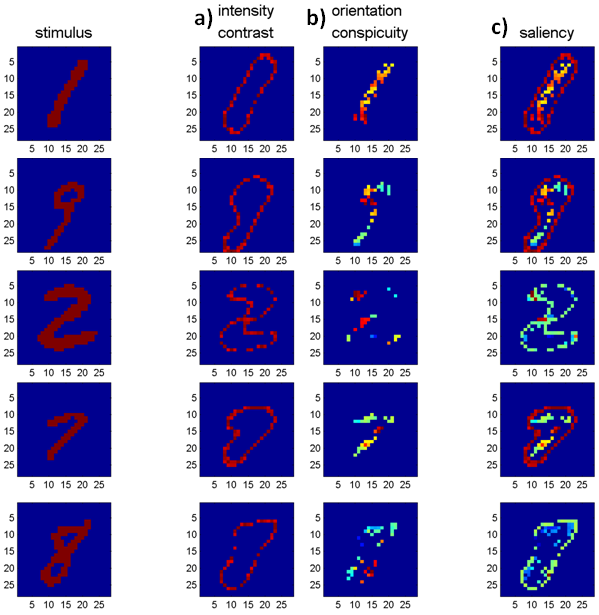
\includegraphics[width=0.8\textwidth]{saliency_examples}
\caption{Examples of saliency maps generated from handwritten digits from the MNIST database\cref{LeCun1998}, where columns depict \textbf{a)} intensity contrast; response to convovling stimuli with a Difference of Gaussians kernel, \textbf{b)} orientation conspicuity; local variance of a pixel's preferred orientation relative to neighboring pixels, \textbf{c)} stimulus map of input stimuli; linear combination of intensity contrast and orientation conspicuity.
\label{fig:saliency_examples}}
\end{figure}

The selection of the attention window is determined through a stochasitc process. This non-deterministic process may mitigate the problem of locking onto the same region during successive sampling events, thus increasing the chance of delivering more diverse information to the recognition system. 

\begin{figure}[ht]
\centering
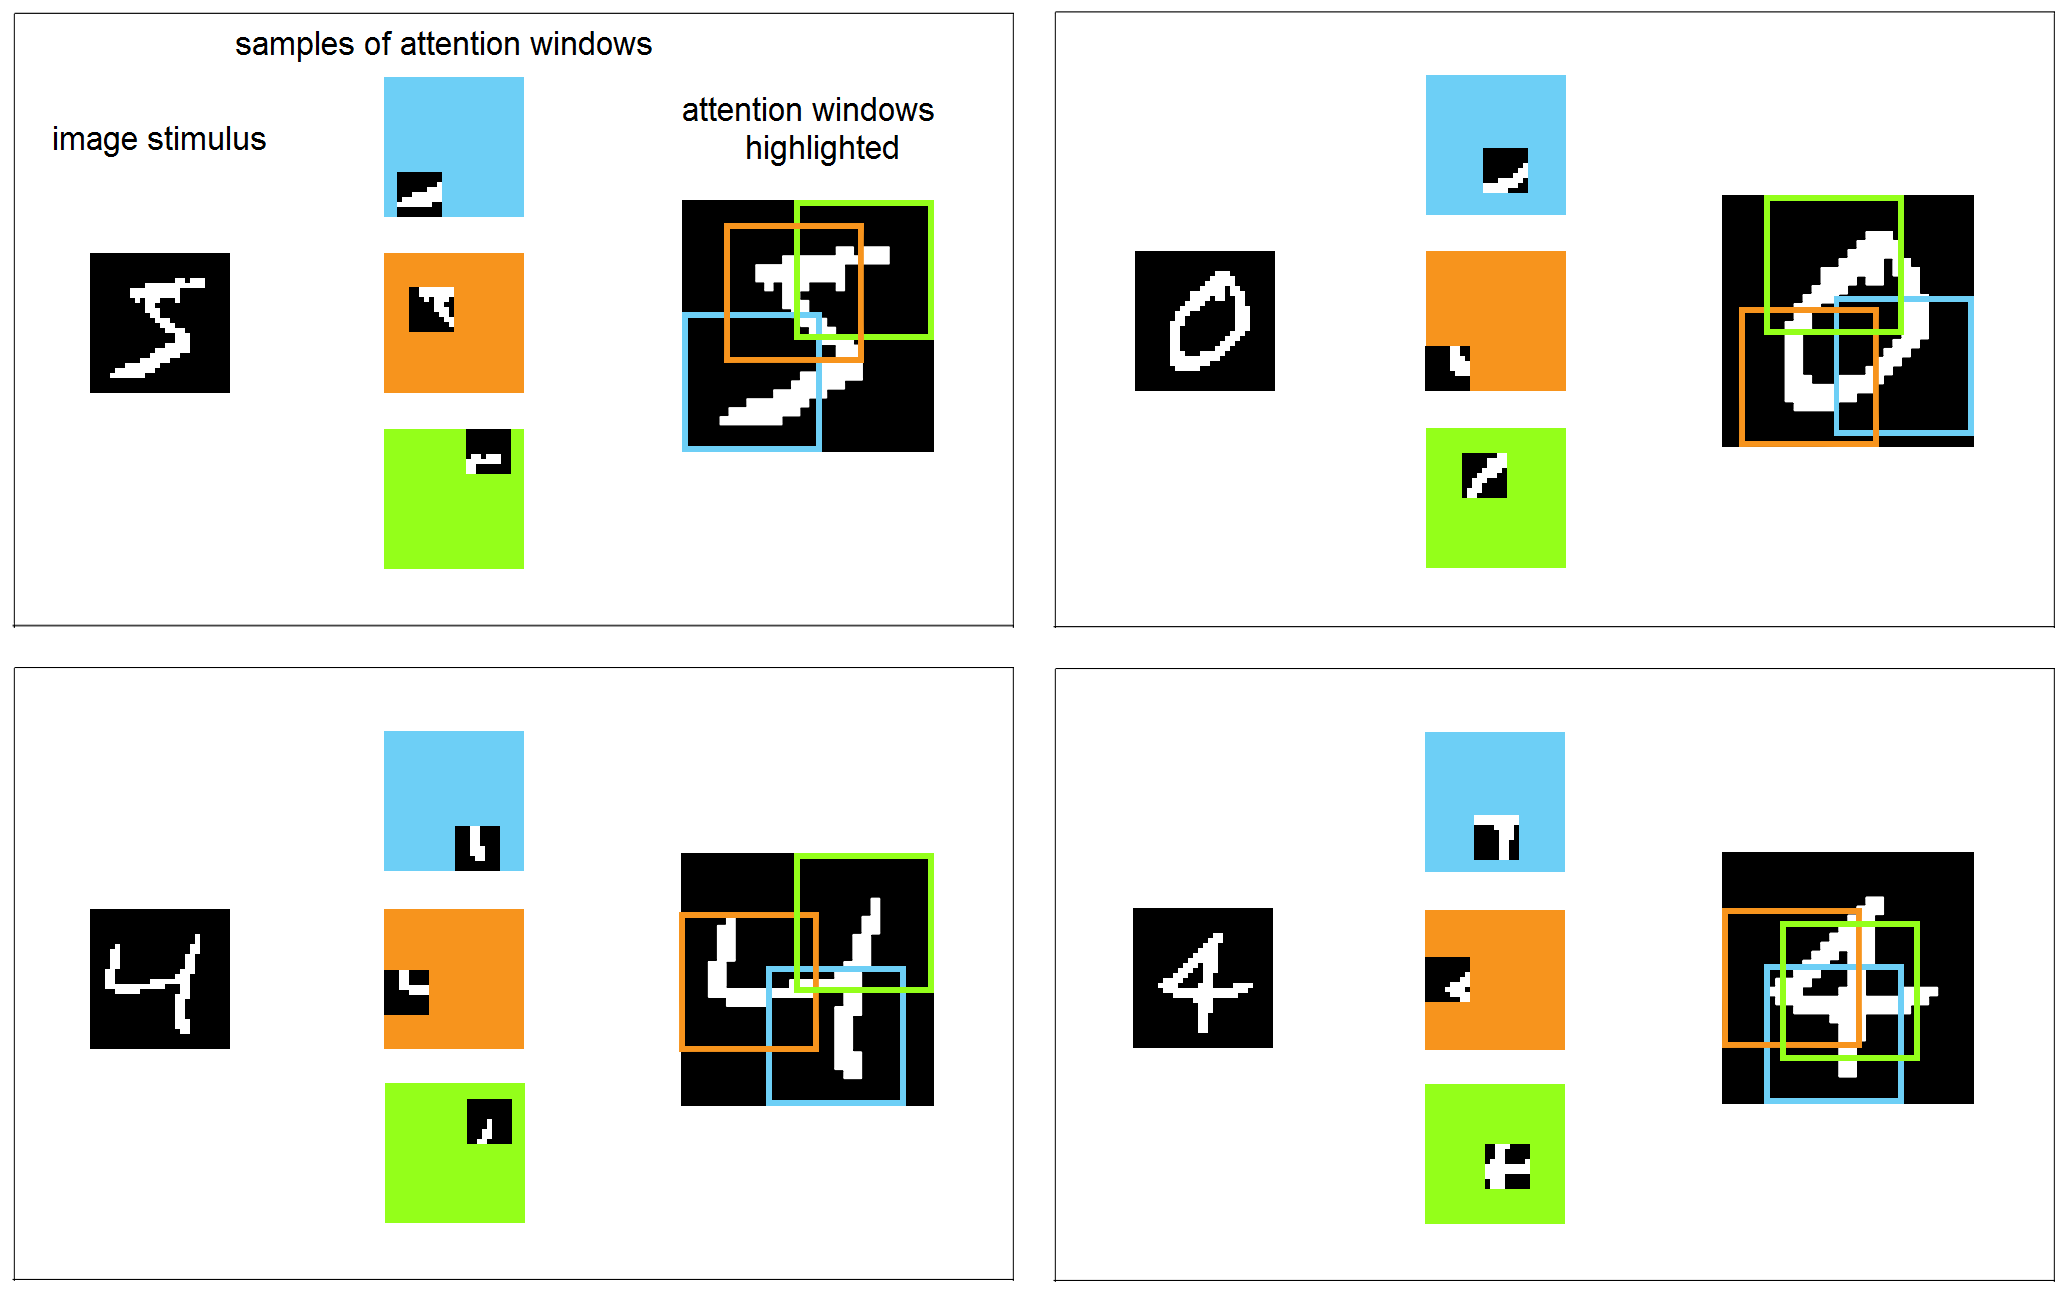
\includegraphics[width=0.8\textwidth]{attention_windows_examples}
\caption{Examples of attention windows determined by sampling from a two-dimensional saliency distribution.
\label{fig:attention_windows_examples}}
\end{figure}

\subsection{The F-layer}

The injection of an intermediate layer that actvates $z$ neurons in the output layer provides a reduction of dimensionality for these neurons and exploits the input provided from the attention mechanism. This layer is mainly concerned with learning abstract geometrical shapes based on low level features such as intensities and orientation maps. 

\chapter{Discussion}

\chapter{Conclusion}

That's all folks!

\chapter{Acknowledgments}

Michael
My family: Sahra, father
My friends Malte Alf
Matthew Cook
INI

\appendix

\chapter{The First Appendix}

The \verb"\appendix" command should be used only once. Subsequent appendices can
be created using the Chapter command.

\chapter{The Second Appendix}

Some text for the second Appendix.

\bibliographystyle{plain}
\bibliography{collection}

\end{document}
